% Ce fichier main.tex est le fichier principal \`{a} partir duquel tout est g\'{e}n\'{e}r\'{e}
%This file is the main file where the final document is generated
%appel de la class these-ubl 
% these-ubl class call
\documentclass{these-ubl} 
\usepackage{biblatex}
\addbibresource{./biblio/biblio.bib}
\geometry{vmargin=4.0cm}
%Pour diff\'{e}rentes universit\'{e}s il faurdra modifier ce d\'{e}but de document
%For different universities modify the beginning of this document to adapt the logos (logo)
\geometry{vmargin=4.0cm}
\logoecoledoc{./Couverture-these/MathSTIC/logo-mathSTIC} %logo ecole doctorale
\logoetablissement{./Couverture-these/MathSTIC/logo-etablissements/logoUR1}%logo etablissement (ici Rennes 1)
\vspace{2.5cm}
%Indiquer l'\'{e}tablissement de d\'{e}livrance du diplome
%Provide the name of the institution that delivers the diploma, 
\unite{L'UNIVERSIT\'{E} DE RENNES 1}
%Si la th\`{e}se est en co-tutelle ou en d\'{e}livrance conjointe, mettre le logo des 2 \'{e}tablissements 
%in the case of "co-tutelle" provide both names (logos)
\ubl{Comue Université Bretagne Loire}
%Indiquer le num\'{e}ro d’accr\'{e}ditation de l’\'{e}cole doctorale de r\'{e}f\'{e}rence pour la th\`{e}se 
%indicate the certification number of l'ecole doctorale
\ecoledoc{\'{E}cole Doctorale N° 601}
%Indiquer le nom de l’\'{e}cole doctorale de r\'{e}f\'{e}rence pour la th\`{e}se 
%Indicate the name of l'ecole doctorale
\nomecole{Math\'{e}matiques et Sciences et Technologies \\ de l'Information et de la Communication}
%Inscrivez ici votre sp\'{e}cialit\'{e} (voir liste des sp\'{e}cialit\'{e}s sur le site de votre \'{e}cole doctorale)
%Indicate the domain (see list of domains in your ecole doctorale)
\spec{Sp\'{e}cialit\'{e} : \textit{(voir liste des sp\'{e}cialit\'{e}s)}}
\usepackage{eso-pic}


\begin{document}
% La page de garde est en français
% The front cover is in French
\selectlanguage{french}

%background image of the front cover
\AddToShipoutPicture*{%
    \put(0,0){%
    \parbox[b][42.5cm]{\paperwidth}{%
        \vfill
        
\includegraphics[width=\paperwidth,keepaspectratio]{./Couverture-these/MathSTIC/image-fond-MATHSTIC-garde.pdf}% image de fond UR1
        \vfill
}}}
%Attention : le pr\'{e}nom doit être en minuscules (Jean) et le NOM en majuscules (BRITTEF) 
%Attention : the first name in small letters and the name in Capital letters 
\author{« Pr\'{e}nom NOM »}
% Donner le titre complet de la th\`{e}se, \'{e}ventuellement le sous titre, si n\'{e}cessaire sur plusieurs lignes 
%Give the complete title of the thesis, if necessary on several lines
\title{« Titre de la th\`{e}se »}
\lesoustitre{« Sous-titre de la th\`{e}se »}
%Indiquer la date et le lieu de soutenance de la th\`{e}se 
%indicates the date and the place of the defense 
\date{« date »}
\lieu{« Lieu »}
%Indiquer le nom du (ou des) laboratoire (s) dans le(s)quel(s) le travail de th\`{e}se a \'{e}t\'{e} effectu\'{e}, indiquer aussi si souhait\'{e} le nom de la (les) facult\'{e}(s) (UFR, \'{e}cole(s), Institut(s), Centre(s)...), son (leurs) adresse(s)... 
%Indicates the name (or names) of research laboratories where the work has been done as well as (if desired) the names of faculties (UFR, Schools, institution...
\uniterecherche{Unit\'{e} de recherche : }
%Indiquer le Numero de th\`{e}se, si cela est opportun, ou faire disparaitre cet item de la couverture 
%Indicate the number of the thesis if there is one.
\numthese{Th\`{e}se N° :  }
%Indiquer le Pr\'{e}nom en minuscules et le Nom en majuscules, le titre de la personne et l’\'{e}tablissement dans lequel il effectue sa recherche  
%Indicates the first name on small letters and the Names on capital letters, the person's title and the institution where he/she belongs to.
%Exemples :  Examples :
%%%- Professeur, Universit\'{e} d’Angers 
%%%- Chercheur, CNRS, \'{e}cole Centrale de Nantes 
%%%-  Professeur d’universit\'{e} – Praticien Hospitalier, Universit\'{e} Paris V  
%%%-  Maitre de conf\'{e}rences, Oniris 
%%%- Charg\'{e} de recherche, INSERM, HDR, Universit\'{e} de Tours  
 %S’il n’y a pas de co-direction, faire disparaitre cet item de la couverture  
 %In there is no co-director, remove the item from the cover


\jury{
{\normalsize \textbf{Rapporteurs avant soutenance :}}\\ \newline
\footnotesize
\begin{tabular}{@{}ll}
Pr\'{e}nom Nom & Fonction et \'{e}tablissement d'exercice \\
Pr\'{e}nom Nom & Fonction et \'{e}tablissement d'exercice \\
Pr\'{e}nom Nom & Fonction et \'{e}tablissement d'exercice \\
\end{tabular}

\vspace{\baselineskip}
{\normalsize \textbf{Composition du Jury :}}\\
{\fontsize{9.5}{11}\selectfont {\textcolor{red}{\textit{Attention, en cas d’absence d’un des membres du Jury le jour de la soutenance, la composition du jury doit être revue pour s’assurer qu’elle est conforme et devra être répercutée sur la couverture de thèse}}}}\\ \newline
\footnotesize
\begin{tabular}{@{}lll}

Pr\'{e}sident :        & Pr\'{e}nom Nom & Fonction et \'{e}tablissement d'exercice \textit{(à préciser après la soutenance)} \\
Examinateurs :         & Pr\'{e}nom Nom & Fonction et \'{e}tablissement d'exercice \\
                       & Pr\'{e}nom Nom & Fonction et \'{e}tablissement d'exercice \\
                       & Pr\'{e}nom Nom & Fonction et \'{e}tablissement d'exercice \\
                       & Pr\'{e}nom Nom & Fonction et \'{e}tablissement d'exercice \\
Dir. de th\`{e}se :    & Pr\'{e}nom Nom & Fonction et \'{e}tablissement d'exercice \\
Co-dir. de th\`{e}se : & Pr\'{e}nom Nom & Fonction et \'{e}tablissement d'exercice \textit{(si pertinent)} \\
\end{tabular}

\vspace{\baselineskip}
{\normalsize \textbf{Invit\'{e}(s) :}}\\
\footnotesize
\begin{tabular}{@{}ll}
Pr\'{e}nom Nom & Fonction et \'{e}tablissement d'exercice \\
\end{tabular}
}


\maketitle
 % page de garde UR1

%\clearemptydoublepage
%inclusion du chapitre remerciement (acknowledgement)
%input acknowledgement chapter 
\chapter*{Acknowledgement}

Je tiens à remercier  \\
I would like to thank. my parents..\\
J'adresse également toute ma reconnaissance à .... \\
....

%stopcover evite d'avoir l'image de fond sur tout le document
%stopcover remove the background image in the rest of the document.
%ce .tex sert \`{a} arr\^{e}ter l'image de fond de la couverture
%This file avoids to have the cover background in all the document.
\ClearShipoutPicture
\thispagestyle{empty}
\clearemptydoublepage
% Ne pas oublier cette commande qui g\'{e}n\`{e}re la page de couverture avant
%This command will generate the front cover
\frontmatter 
\renewcommand{\contentsname}{Table of Contents}
\tableofcontents %sommaire %table of content


\chapter*{Introduction}
\addcontentsline{toc}{chapter}{Introduction}
\chaptermark{Introduction}


Lorem ipsum dolor sit amet, «~consectetuer~» adipiscing elit. Maecenas fermentum, elit non lobortis cursus, orci velit suscipit est, id mollis turpis mi eget orci. Ut aliquam sollicitudin metus. Mauris at sapien sed sapien congue iaculis. Nulla lorem urna, bibendum id, laoreet iaculis, nonummy eget, massa. Phasellus ullamcorper commodo velit. Class aptent taciti sociosqu ad litora torquent per «~conubia nostra~», per inceptos hymenaeos. Phasellus est. Maecenas felis augue, gravida quis, porta adipiscing, iaculis vitae, felis. Nullam ipsum. Nulla a sem ac leo fringilla mattis. Phasellus egestas augue in sem. Etiam ac enim non mauris ullamcorper scelerisque. In wisi leo, malesuada vulputate, tempor sit amet, facilisis vel, velit. Mauris massa est, sodales placerat, luctus id, hendrerit a, urna. Nullam eleifend pede eget odio. Duis non erat. Nullam pellentesque.

\begin{verse}
Maître Corbeau, sur un arbre perché, \\
Tenait en son bec un fromage. \\
Maître Renard, par l'odeur alléché, \\
Lui tint à peu près ce langage : \\
«~Hé ! bonjour, Monsieur du Corbeau. \\
Que vous êtes joli ! que vous me semblez beau ! \\
Sans mentir, si votre ramage \\
Se rapporte à votre plumage, \\
Vous êtes le Phénix des hôtes de ces bois.~» \\
\end{verse}

Lorem ipsum dolor sit amet, consectetuer adipiscing elit. Maecenas fermentum, elit non lobortis cursus, orci velit suscipit est, id mollis turpis mi eget orci. Ut aliquam sollicitudin metus. Mauris at sapien sed sapien congue iaculis. Nulla lorem urna, bibendum id, laoreet iaculis, nonummy eget, massa\footcite[32]{Pierre1901}. Phasellus ullamcorper commodo velit. Class aptent taciti sociosqu ad litora torquent per conubia nostra, per inceptos hymenaeos. Phasellus est. Maecenas felis augue, gravida quis, porta adipiscing, iaculis vitae, felis. Nullam ipsum. Nulla a sem ac leo fringilla mattis. Phasellus egestas augue in sem. Etiam ac enim non mauris ullamcorper scelerisque. In wisi leo, malesuada vulputate, tempor sit amet, facilisis vel, velit. Mauris massa est, sodales placerat, luctus id, hendrerit a, urna. Nullam eleifend pede eget odio. Duis non erat. Nullam pellentesque. 

\section*{Première section de l'intro}
\addcontentsline{toc}{section}{Première section de l'intro}

Lorem ipsum dolor sit amet, «~consectetuer~» adipiscing elit. Maecenas fermentum, elit non lobortis cursus, orci velit suscipit est, id mollis turpis mi eget orci. Ut aliquam sollicitudin metus. Mauris at sapien sed sapien congue iaculis. Nulla lorem urna, bibendum id, laoreet iaculis, nonummy eget, massa. Phasellus ullamcorper commodo velit. Class aptent taciti sociosqu ad litora torquent per «~conubia nostra~», per inceptos hymenaeos. Phasellus est. Maecenas felis augue, gravida quis, porta adipiscing, iaculis vitae, felis. Nullam ipsum. Nulla a sem ac leo fringilla mattis. Phasellus egestas augue in sem. Etiam ac enim non mauris ullamcorper scelerisque. In wisi leo, malesuada vulputate, tempor sit amet, facilisis vel, velit. Mauris massa est, sodales placerat, luctus id, hendrerit a, urna. Nullam eleifend pede eget odio. Duis non erat. Nullam pellentesque.

\textbf{Une boite magique : }

\boitemagique{Titre de la boite}{
Praesent placerat, ante at venenatis pretium, diam turpis faucibus arcu, nec vehicula quam lorem ut leo. Sed facilisis, augue in pharetra dapibus, ligula justo accumsan massa, eu suscipit felis ipsum eget enim.
}

Laoreet iaculis, nonummy eget, massa. Phasellus ullamcorper commodo velit. Class aptent taciti sociosqu ad litora torquent per «~conubia nostra~», per inceptos hymenaeos. Phasellus est. Maecenas felis augue, gravida quis, porta adipiscing, iaculis vitae, felis. Nullam ipsum. Nulla a sem ac leo fringilla mattis. Phasellus egestas augue in sem. Etiam ac enim non mauris ullamcorper scelerisque. In wisi leo, malesuada vulputate, tempor sit amet, facilisis vel, velit. Mauris massa est, sodales placerat, luctus id, hendrerit a, urna. Nullam eleifend pede eget odio. Duis non erat. Nullam pellentesque.

\textbf{Une boite simple : }
\boitesimple{Mauris lorem quam, tristique sollicitudin egestas sed, sodales vel leo. In hac habitasse platea dictumst. Lorem ipsum dolor sit amet, consectetur adipiscing elit. Sed sed lorem lacus, at venenatis elit. Pellentesque nisl arcu, blandit ac eleifend non, sodales a quam.}

Laoreet iaculis, nonummy eget, massa. Phasellus ullamcorper commodo velit. Class aptent taciti sociosqu ad litora torquent per «~conubia nostra~», per inceptos hymenaeos. Phasellus est. Maecenas felis augue, gravida quis, porta adipiscing, iaculis vitae, felis. Nullam ipsum. Nulla a sem ac leo fringilla mattis. Phasellus egestas augue in sem. Etiam ac enim non mauris ullamcorper scelerisque. In wisi leo, malesuada vulputate, tempor sit amet, facilisis vel, velit. Mauris massa est, sodales placerat, luctus id, hendrerit a, urna. Nullam eleifend pede eget odio. Duis non erat. Nullam pellentesque.



\clearemptydoublepage
\clearemptydoublepage
%\shorttableofcontents{Sommaire}{0}
%
% Mettre ici votre chapitre d'Introduction, le cas \'{e}ch\'{e}ant
%Input the introduction chapter 
% 
\clearemptydoublepage
\mainmatter % Ne pas oublier, avec \frontmatter et \backmatter
	           %this command inputs \frontmatter and \backmatter as a cover in the front and the back
%
% Mettre ici votre chapitre 1
%Input your chapter 1
%

\clearemptydoublepage
\chapter{Titre du premier chapitre}

Lorem ipsum dolor sit amet, «~consectetuer~» adipiscing elit. Maecenas fermentum, elit non lobortis cursus, orci velit suscipit est, id mollis turpis mi eget orci. Ut aliquam sollicitudin metus. Mauris at sapien sed sapien congue iaculis. Nulla lorem urna, bibendum id, laoreet iaculis, nonummy eget, massa. Phasellus ullamcorper commodo velit. Class aptent taciti sociosqu ad litora torquent per «~conubia nostra~», per inceptos hymenaeos. Phasellus est. Maecenas felis augue, gravida quis, porta adipiscing, iaculis vitae, felis. Nullam ipsum. Nulla a sem ac leo fringilla mattis. Phasellus egestas augue in sem. Etiam ac enim non mauris ullamcorper scelerisque. In wisi leo, malesuada vulputate, tempor sit amet, facilisis vel, velit. Mauris massa est, sodales placerat, luctus id, hendrerit a, urna. Nullam eleifend pede eget odio. Duis non erat. Nullam pellentesque.

Lorem ipsum dolor sit amet, consectetuer adipiscing elit. Maecenas fermentum, elit non lobortis cursus, orci velit suscipit est, id mollis turpis mi eget orci. Ut aliquam sollicitudin metus. Mauris at sapien sed sapien congue iaculis. Nulla lorem urna, bibendum id, laoreet iaculis, nonummy eget, massa\footcite[12]{Pierre1901}. Phasellus ullamcorper commodo velit. Class aptent taciti sociosqu ad litora torquent per conubia nostra, per inceptos hymenaeos. Phasellus est. Maecenas felis augue, gravida quis, porta adipiscing, iaculis vitae, felis. Nullam ipsum. Nulla a sem ac leo fringilla mattis. Phasellus egestas augue in sem. Etiam ac enim non mauris ullamcorper scelerisque. In wisi leo, malesuada vulputate, tempor sit amet, facilisis vel, velit. Mauris massa est, sodales placerat, luctus id, hendrerit a, urna. Nullam eleifend pede eget odio. Duis non erat. Nullam pellentesque. 

\section{Première section du chapitre}

\subsection{Première sous-section}

Cras molestie. Curabitur id urna. Suspendisse tempor. Aliquam erat volutpat. Aliquam erat volutpat. Nam ultricies metus sit amet erat\footnote{Mauris neque odio, ornare id, rhoncus non, sollicitudin sed, lectus. Phasellus et dolor. Aenean ullamcorper risus id libero. Pellentesque ac sem eget libero aliquam tincidunt. Suspendisse neque.}. Suspendisse eget ipsum ut purus imperdiet suscipit. Mauris sed urna at diam volutpat placerat. Nulla vitae tortor. Nulla sed nisl.

Lorem ipsum dolor sit amet, consectetuer adipiscing elit. Maecenas fermentum, elit non lobortis cursus, orci velit suscipit est, id mollis turpis mi eget orci. Ut aliquam sollicitudin metus. Mauris at sapien sed sapien congue iaculis. Nulla lorem urna, bibendum id, laoreet iaculis, nonummy eget, massa. Phasellus ullamcorper commodo velit. Class aptent taciti sociosqu ad litora torquent per conubia nostra, per inceptos hymenaeos. Phasellus est. Maecenas felis augue, gravida quis, porta adipiscing, iaculis vitae, felis. Nullam ipsum. Nulla a sem ac leo fringilla mattis. Phasellus egestas augue in sem. Etiam ac enim non mauris ullamcorper scelerisque. In wisi leo, malesuada vulputate, tempor sit amet, facilisis vel, velit. Mauris massa est, sodales placerat, luctus id, hendrerit a, urna. Nullam eleifend pede eget odio. Duis non erat. Nullam pellentesque\footcite[56]{Desfois1998}.


\begin{quote}
Aenean ullamcorper risus id libero. Pellentesque ac sem eget libero aliquam tincidunt. Suspendisse neque. Rutrum id, faucibus vitae, leo. Donec ut wisi. Vivamus ornare, lorem quis tristique dapibus, nulla nisl nonummy libero, vitae luctus sem felis vel nisl. Suspendisse lectus lacus, ultricies vitae, feugiat et, hendrerit in, quam. Pellentesque porttitor enim at lectus. Praesent viverra laoreet velit. Mauris neque odio, ornare id, rhoncus non, sollicitudin sed, lectus. Aenean ullamcorper risus id libero. Pellentesque ac sem eget libero aliquam tincidunt. Suspendisse neque\footcite[voir \pno~154]{Georges1974}.
\end{quote}



Morbi lorem. Etiam scelerisque rhoncus orci\footcite{Georges1974}. Nunc elementum ante ac leo. Vestibulum venenatis dictum nunc. Donec turpis est, dictum nec, fringilla nec, cursus id, quam. In nibh orci, porttitor ut, rutrum id, faucibus vitae, leo. Donec ut wisi. Vivamus ornare, lorem quis tristique dapibus, nulla nisl nonummy libero, vitae luctus sem felis vel nisl. Suspendisse lectus lacus, ultricies vitae, feugiat et, hendrerit in, quam. Pellentesque porttitor enim at lectus. Praesent viverra laoreet velit\footcite[56]{Desfois1998}. Mauris neque odio, ornare id, rhoncus non, sollicitudin sed, lectus. Phasellus et dolor. Aenean ullamcorper risus id libero. Pellentesque ac sem eget libero aliquam tincidunt. Suspendisse neque. Curabitur egestas neque ultrices nisl. Nulla bibendum augue et tellus. Duis ultrices convallis est.



Lorem ipsum dolor sit amet, consectetuer adipiscing elit. Maecenas fermentum, elit non lobortis cursus, orci velit suscipit est, id mollis turpis mi eget orci. Ut aliquam sollicitudin metus. Mauris at sapien sed sapien congue iaculis. Nulla lorem urna, bibendum id, laoreet iaculis, nonummy eget, massa. Phasellus ullamcorper commodo velit. Class aptent taciti sociosqu ad litora torquent per conubia nostra, per inceptos hymenaeos. Phasellus est. Maecenas felis augue, gravida quis, porta adipiscing, iaculis vitae, felis. Nullam ipsum. Nulla a sem ac leo fringilla mattis. Phasellus egestas augue in sem. Etiam ac enim non mauris ullamcorper scelerisque. In wisi leo, malesuada vulputate, tempor sit amet, facilisis vel, velit. Mauris massa est, sodales placerat, luctus id, hendrerit a, urna. Nullam eleifend pede eget odio. Duis non erat. Nullam pellentesque.

Lorem ipsum dolor sit amet, consectetuer adipiscing elit. Maecenas fermentum, elit non lobortis cursus, orci velit suscipit est, id mollis turpis mi eget orci. Ut aliquam sollicitudin metus. Mauris at sapien sed sapien congue iaculis. Nulla lorem urna, bibendum id, laoreet iaculis, nonummy eget, massa. Phasellus ullamcorper commodo velit. Class aptent taciti sociosqu ad litora torquent per conubia nostra, per inceptos hymenaeos. Phasellus est. Maecenas felis augue, gravida quis, porta adipiscing, iaculis vitae, felis. Nullam ipsum. Nulla a sem ac leo fringilla mattis. Phasellus egestas augue in sem. Etiam ac enim non mauris ullamcorper scelerisque. In wisi leo, malesuada vulputate, tempor sit amet, facilisis vel, velit. Mauris massa est, sodales placerat, luctus id, hendrerit a, urna. Nullam eleifend pede eget odio. Duis non erat. Nullam pellentesque.
Voir figure \ref{fig:mafigure2}.


\begin{figure}[htbp]
   \begin{center}
      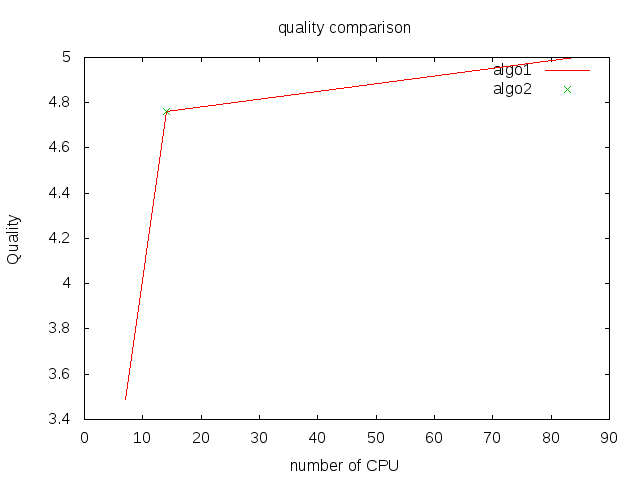
\includegraphics[width=0.8\linewidth]{Chapitre1/figures/comparison.png}
   \end{center}
   \caption[titre court pour la liste des figures]
   {\footnotesize Titre plus long avec des explications.}
   \label{fig:mafigure2}
\end{figure}


\subsection{Deuxième sous-section}

Morbi lorem. Etiam scelerisque rhoncus orci. Nunc elementum ante ac leo. Vestibulum venenatis dictum nunc. Donec turpis est, dictum nec, fringilla nec, cursus id, quam. In nibh orci, porttitor ut, rutrum id, faucibus vitae, leo. Donec ut wisi. Vivamus ornare, lorem quis tristique dapibus, nulla nisl nonummy libero, vitae luctus sem felis vel nisl. Suspendisse lectus lacus, ultricies vitae, feugiat et, hendrerit in, quam. Pellentesque porttitor enim at lectus. Praesent viverra laoreet velit. Mauris neque odio, ornare id, rhoncus non, sollicitudin sed, lectus. Phasellus et dolor. Aenean ullamcorper risus id libero. Pellentesque ac sem eget libero aliquam tincidunt. Suspendisse neque. Curabitur egestas neque ultrices nisl. Nulla bibendum augue et tellus. Duis ultrices convallis est.

Lorem ipsum dolor sit amet, consectetuer adipiscing elit. Maecenas fermentum, elit non lobortis cursus, orci velit suscipit est, id mollis turpis mi eget orci. Ut aliquam sollicitudin metus. Mauris at sapien sed sapien congue iaculis. Nulla lorem urna, bibendum id, laoreet iaculis, nonummy eget, massa. Phasellus ullamcorper commodo velit. Class aptent taciti sociosqu ad litora torquent per conubia nostra, per inceptos hymenaeos. Phasellus est. Maecenas felis augue, gravida quis, porta adipiscing, iaculis vitae, felis. Nullam ipsum. Nulla a sem ac leo fringilla mattis. Phasellus egestas augue in sem. Etiam ac enim non mauris ullamcorper scelerisque. In wisi leo, malesuada vulputate, tempor sit amet, facilisis vel, velit. Mauris massa est, sodales placerat, luctus id, hendrerit a, urna. Nullam eleifend pede eget odio. Duis non erat. Nullam pellentesque.

Lorem ipsum dolor sit amet, consectetuer adipiscing elit. Maecenas fermentum, elit non lobortis cursus, orci velit suscipit est, id mollis turpis mi eget orci. Ut aliquam sollicitudin metus. Mauris at sapien sed sapien congue iaculis. Nulla lorem urna, bibendum id, laoreet iaculis, nonummy eget, massa. Phasellus ullamcorper commodo velit. Class aptent taciti sociosqu ad litora torquent per conubia nostra, per inceptos hymenaeos. Phasellus est. Maecenas felis augue, gravida quis, porta adipiscing, iaculis vitae, felis. Nullam ipsum. Nulla a sem ac leo fringilla mattis. Phasellus egestas augue in sem. Etiam ac enim non mauris ullamcorper scelerisque. In wisi leo, malesuada vulputate, tempor sit amet, facilisis vel, velit. Mauris massa est, sodales placerat, luctus id, hendrerit a, urna. Nullam eleifend pede eget odio. Duis non erat. Nullam pellentesque.

Lorem ipsum dolor sit amet, consectetuer adipiscing elit. Maecenas fermentum, elit non lobortis cursus, orci velit suscipit est, id mollis turpis mi eget orci. Ut aliquam sollicitudin metus. Mauris at sapien sed sapien congue iaculis. Nulla lorem urna, bibendum id, laoreet iaculis, nonummy eget, massa. Phasellus ullamcorper commodo velit. Class aptent taciti sociosqu ad litora torquent per conubia nostra, per inceptos hymenaeos. Phasellus est. Maecenas felis augue, gravida quis, porta adipiscing, iaculis vitae, felis. Nullam ipsum. Nulla a sem ac leo fringilla mattis. Phasellus egestas augue in sem. Etiam ac enim non mauris ullamcorper scelerisque. In wisi leo, malesuada vulputate, tempor sit amet, facilisis vel, velit. Mauris massa est, sodales placerat, luctus id, hendrerit a, urna. Nullam eleifend pede eget odio. Duis non erat. Nullam pellentesque.

Lorem ipsum dolor sit amet, consectetuer adipiscing elit. Maecenas fermentum, elit non lobortis cursus, orci velit suscipit est, id mollis turpis mi eget orci. Ut aliquam sollicitudin metus. Mauris at sapien sed sapien congue iaculis. Nulla lorem urna, bibendum id, laoreet iaculis, nonummy eget, massa. Phasellus ullamcorper commodo velit. Class aptent taciti sociosqu ad litora torquent per conubia nostra, per inceptos hymenaeos. Phasellus est. Maecenas felis augue, gravida quis, porta adipiscing, iaculis vitae, felis. Nullam ipsum. Nulla a sem ac leo fringilla mattis. Phasellus egestas augue in sem. Etiam ac enim non mauris ullamcorper scelerisque. In wisi leo, malesuada vulputate, tempor sit amet, facilisis vel, velit. Mauris massa est, sodales placerat, luctus id, hendrerit a, urna. Nullam eleifend pede eget odio. Duis non erat. Nullam pellentesque.

Lorem ipsum dolor sit amet, «~consectetuer~» adipiscing elit. Maecenas fermentum, elit non lobortis cursus, orci velit suscipit est, id mollis turpis mi eget orci. Ut aliquam sollicitudin metus. Mauris at sapien sed sapien congue iaculis. Nulla lorem urna, bibendum id, laoreet iaculis, nonummy eget, massa. Phasellus ullamcorper commodo velit. Class aptent taciti sociosqu ad litora torquent per «~conubia nostra~», per inceptos hymenaeos. Phasellus est. Maecenas felis augue, gravida quis, porta adipiscing, iaculis vitae, felis. Nullam ipsum. Nulla a sem ac leo fringilla mattis. Phasellus egestas augue in sem. Etiam ac enim non mauris ullamcorper scelerisque. In wisi leo, malesuada vulputate, tempor sit amet, facilisis vel, velit. Mauris massa est, sodales placerat, luctus id, hendrerit a, urna. Nullam eleifend pede eget odio. Duis non erat. Nullam pellentesque.

Lorem ipsum dolor sit amet, «~consectetuer~» adipiscing elit. Maecenas fermentum, elit non lobortis cursus, orci velit suscipit est, id mollis turpis mi eget orci. Ut aliquam sollicitudin metus. Mauris at sapien sed sapien congue iaculis. Nulla lorem urna, bibendum id, laoreet iaculis, nonummy eget, massa. Phasellus ullamcorper commodo velit. Class aptent taciti sociosqu ad litora torquent per «~conubia nostra~», per inceptos hymenaeos. Phasellus est. Maecenas felis augue, gravida quis, porta adipiscing, iaculis vitae, felis. Nullam ipsum. Nulla a sem ac leo fringilla mattis. Phasellus egestas augue in sem. Etiam ac enim non mauris ullamcorper scelerisque. In wisi leo, malesuada vulputate, tempor sit amet, facilisis vel, velit. Mauris massa est, sodales placerat, luctus id, hendrerit a, urna. Nullam eleifend pede eget odio. Duis non erat. Nullam pellentesque.

Lorem ipsum dolor sit amet, «~consectetuer~» adipiscing elit. Maecenas fermentum, elit non lobortis cursus, orci velit suscipit est, id mollis turpis mi eget orci. Ut aliquam sollicitudin metus. Mauris at sapien sed sapien congue iaculis. Nulla lorem urna, bibendum id, laoreet iaculis, nonummy eget, massa. Phasellus ullamcorper commodo velit. Class aptent taciti sociosqu ad litora torquent per «~conubia nostra~», per inceptos hymenaeos. Phasellus est. Maecenas felis augue, gravida quis, porta adipiscing, iaculis vitae, felis. Nullam ipsum. Nulla a sem ac leo fringilla mattis. Phasellus egestas augue in sem. Etiam ac enim non mauris ullamcorper scelerisque. In wisi leo, malesuada vulputate, tempor sit amet, facilisis vel, velit. Mauris massa est, sodales placerat, luctus id, hendrerit a, urna. Nullam eleifend pede eget odio. Duis non erat. Nullam pellentesque.


\section{Conclusion du premier chapitre}


Lorem ipsum dolor sit amet, consectetuer adipiscing elit. Maecenas fermentum, elit non lobortis cursus, orci velit suscipit est, id mollis turpis mi eget orci. Ut aliquam sollicitudin metus. Mauris at sapien sed sapien congue iaculis. Nulla lorem urna, bibendum id, laoreet iaculis, nonummy eget, massa. Phasellus ullamcorper commodo velit. Class aptent taciti sociosqu ad litora torquent per conubia nostra, per inceptos hymenaeos. Phasellus est. Maecenas felis augue, gravida quis, porta adipiscing, iaculis vitae, felis. Nullam ipsum. Nulla a sem ac leo fringilla mattis. Phasellus egestas augue in sem. Etiam ac enim non mauris ullamcorper scelerisque. In wisi leo, malesuada vulputate, tempor sit amet, facilisis vel, velit. Mauris massa est, sodales placerat, luctus id, hendrerit a, urna. Nullam eleifend pede eget odio. Duis non erat. Nullam pellentesque.


%
% Mettre ici votre chapitre 2
%Input your chapter 2
% 
\clearemptydoublepage

\chapter[ceci est un long titre]{Nom du chapitre 2}

Lorem ipsum dolor sit amet, «~consectetuer~» adipiscing elit. Maecenas fermentum, elit non lobortis cursus, orci velit suscipit est, id mollis turpis mi eget orci. Ut aliquam sollicitudin metus. Mauris at sapien sed sapien congue iaculis. Nulla lorem urna, bibendum id, laoreet iaculis, nonummy eget, massa. Phasellus ullamcorper commodo velit. Class aptent taciti sociosqu ad litora torquent per «~conubia nostra~», per inceptos hymenaeos. Phasellus est. Maecenas felis augue, gravida quis, porta adipiscing, iaculis vitae, felis. Nullam ipsum. Nulla a sem ac leo fringilla mattis. Phasellus egestas augue in sem. Etiam ac enim non mauris ullamcorper scelerisque. In wisi leo, malesuada vulputate, tempor sit amet, facilisis vel, velit. Mauris massa est, sodales placerat, luctus id, hendrerit a, urna. Nullam eleifend pede eget odio. Duis non erat. Nullam pellentesque\footcite[225]{Doule1887}.

\section{Première section du chapitre}

\subsection{Première sous-section}

Cras molestie. Curabitur id urna. Suspendisse tempor. Aliquam erat volutpat. Aliquam erat volutpat. Nam ultricies metus sit amet erat\footnote{Mauris neque odio, ornare id, rhoncus non, sollicitudin sed, lectus. Phasellus et dolor. Aenean ullamcorper risus id libero. Pellentesque ac sem eget libero aliquam tincidunt. Suspendisse neque.}. Suspendisse eget ipsum ut purus imperdiet suscipit. Mauris sed urna at diam volutpat placerat. Nulla vitae tortor. Nulla sed nisl.

Morbi lorem. Etiam scelerisque rhoncus orci. Nunc elementum ante ac leo. Vestibulum venenatis dictum nunc. Donec turpis est, dictum nec\footcite[228]{Drocher2006}, fringilla nec, cursus id, quam. In nibh orci, porttitor ut, rutrum id, faucibus vitae, leo. Donec ut wisi. Vivamus ornare, lorem quis tristique dapibus, nulla nisl nonummy libero, vitae luctus sem felis vel nisl. Suspendisse lectus lacus, ultricies vitae, feugiat et, hendrerit in, quam. Pellentesque porttitor enim at lectus. Praesent viverra laoreet velit. Mauris neque odio, ornare id, rhoncus non, sollicitudin sed, lectus. Phasellus et dolor. Aenean ullamcorper risus id libero. Pellentesque ac sem eget libero aliquam tincidunt. Suspendisse neque. Curabitur egestas neque ultrices nisl. Nulla bibendum augue et tellus. Duis ultrices convallis est.

Lorem ipsum dolor sit amet, consectetuer adipiscing elit. Maecenas fermentum, elit non lobortis cursus, orci velit suscipit est, id mollis turpis mi eget orci. Ut aliquam sollicitudin metus. Mauris at sapien sed sapien congue iaculis. Nulla lorem urna, bibendum id, laoreet iaculis, nonummy eget, massa. Phasellus ullamcorper commodo velit. Class aptent taciti sociosqu ad litora torquent per conubia nostra, per inceptos hymenaeos. Phasellus est. Maecenas felis augue, gravida quis, porta adipiscing, iaculis vitae, felis. Nullam ipsum. Nulla a sem ac leo fringilla mattis. Phasellus egestas augue in sem. Etiam ac enim non mauris ullamcorper scelerisque. In wisi leo, malesuada vulputate, tempor sit amet, facilisis vel, velit. Mauris massa est, sodales placerat, luctus id, hendrerit a, urna. Nullam eleifend pede eget odio. Duis non erat. Nullam pellentesque.


\subsection{Deuxième sous-section}

Morbi lorem. Etiam scelerisque rhoncus orci. Nunc elementum ante ac leo. Vestibulum venenatis dictum nunc. Donec turpis est, dictum nec, fringilla nec, cursus id, quam. In nibh orci, porttitor ut, rutrum id, faucibus vitae, leo. Donec ut wisi. Vivamus ornare, lorem quis tristique dapibus, nulla nisl nonummy libero, vitae luctus sem felis vel nisl. Suspendisse lectus lacus, ultricies vitae, feugiat et, hendrerit in, quam. Pellentesque porttitor enim at lectus. Praesent viverra laoreet velit. Mauris neque odio, ornare id, rhoncus non, sollicitudin sed, lectus. Phasellus et dolor. Aenean ullamcorper risus id libero. Pellentesque ac sem eget libero aliquam tincidunt. Suspendisse neque. Curabitur egestas neque ultrices nisl. Nulla bibendum augue et tellus. Duis ultrices convallis est.

Lorem ipsum dolor sit amet, consectetuer adipiscing elit. Maecenas fermentum, elit non lobortis cursus, orci velit suscipit est, id mollis turpis mi eget orci. Ut aliquam sollicitudin metus. Mauris at sapien sed sapien congue iaculis. Nulla lorem urna, bibendum id, laoreet iaculis, nonummy eget, massa. Phasellus ullamcorper commodo velit. Class aptent taciti sociosqu ad litora torquent per conubia nostra, per inceptos hymenaeos. Phasellus est. Maecenas felis augue, gravida quis, porta adipiscing, iaculis vitae, felis. Nullam ipsum. Nulla a sem ac leo fringilla mattis. Phasellus egestas augue in sem. Etiam ac enim non mauris ullamcorper scelerisque. In wisi leo, malesuada vulputate, tempor sit amet, facilisis vel, velit. Mauris massa est, sodales placerat, luctus id, hendrerit a, urna. Nullam eleifend pede eget odio. Duis non erat. Nullam pellentesque.

Lorem ipsum dolor sit amet, consectetuer adipiscing elit. Maecenas fermentum, elit non lobortis cursus, orci velit suscipit est, id mollis turpis mi eget orci. Ut aliquam sollicitudin metus. Mauris at sapien sed sapien congue iaculis. Nulla lorem urna, bibendum id, laoreet iaculis, nonummy eget, massa. Phasellus ullamcorper commodo velit. Class aptent taciti sociosqu ad litora torquent per conubia nostra, per inceptos hymenaeos. Phasellus est. Maecenas felis augue, gravida quis, porta adipiscing, iaculis vitae, felis. Nullam ipsum. Nulla a sem ac leo fringilla mattis. Phasellus egestas augue in sem. Etiam ac enim non mauris ullamcorper scelerisque. In wisi leo, malesuada vulputate, tempor sit amet, facilisis vel, velit. Mauris massa est, sodales placerat, luctus id, hendrerit a, urna. Nullam eleifend pede eget odio. Duis non erat. Nullam pellentesque.

\section{Conclusion du second chapitre}


Lorem ipsum dolor sit amet, consectetuer adipiscing elit. Maecenas fermentum, elit non lobortis cursus, orci velit suscipit est, id mollis turpis mi eget orci. Ut aliquam sollicitudin metus. Mauris at sapien sed sapien congue iaculis. Nulla lorem urna, bibendum id, laoreet iaculis, nonummy eget, massa. Phasellus ullamcorper commodo velit. Class aptent taciti sociosqu ad litora torquent per conubia nostra, per inceptos hymenaeos. Phasellus est. Maecenas felis augue, gravida quis, porta adipiscing, iaculis vitae, felis. Nullam ipsum. Nulla a sem ac leo fringilla mattis. Phasellus egestas augue in sem. Etiam ac enim non mauris ullamcorper scelerisque. In wisi leo, malesuada vulputate, tempor sit amet, facilisis vel, velit. Mauris massa est, sodales placerat, luctus id, hendrerit a, urna. Nullam eleifend pede eget odio. Duis non erat. Nullam pellentesque.

Lorem ipsum dolor sit amet, consectetuer adipiscing elit. Maecenas fermentum, elit non lobortis cursus, orci velit suscipit est, id mollis turpis mi eget orci. Ut aliquam sollicitudin metus. Mauris at sapien sed sapien congue iaculis. Nulla lorem urna, bibendum id, laoreet iaculis, nonummy eget, massa. Phasellus ullamcorper commodo velit. Class aptent taciti sociosqu ad litora torquent per conubia nostra, per inceptos hymenaeos. Phasellus est. Maecenas felis augue, gravida quis, porta adipiscing, iaculis vitae, felis. Nullam ipsum. Nulla a sem ac leo fringilla mattis. Phasellus egestas augue in sem. Etiam ac enim non mauris ullamcorper scelerisque. In wisi leo, malesuada vulputate, tempor sit amet, facilisis vel, velit. Mauris massa est, sodales placerat, luctus id, hendrerit a, urna. Nullam eleifend pede eget odio. Duis non erat. Nullam pellentesque.

\clearemptydoublepage
%
%
% D\'{e}-commenter pour ins\'{e}rer les autres chapitres, ici votre chapitre X
% Uncomment to insert other chapters, here your chapter X
% 
%\input{./Chapitrex/chapitrex}
%\clearemptydoublepage
% 
\backmatter
\chapter*{Conclusion}
\addcontentsline{toc}{chapter}{Conclusion}
\chaptermark{Conclusion}


Lorem ipsum dolor sit amet, «~consectetuer~» adipiscing elit. Maecenas fermentum, elit non lobortis cursus, orci velit suscipit est, id mollis turpis mi eget orci. Ut aliquam sollicitudin metus. Mauris at sapien sed sapien congue iaculis. Nulla lorem urna, bibendum id, laoreet iaculis, nonummy eget, massa. Phasellus ullamcorper commodo velit. Class aptent taciti sociosqu ad litora torquent per «~conubia nostra~», per inceptos hymenaeos. Phasellus est. Maecenas felis augue, gravida quis, porta adipiscing, iaculis vitae, felis. Nullam ipsum. Nulla a sem ac leo fringilla mattis. Phasellus egestas augue in sem. Etiam ac enim non mauris ullamcorper scelerisque. In wisi leo, malesuada vulputate, tempor sit amet, facilisis vel, velit. Mauris massa est, sodales placerat, luctus id, hendrerit a, urna. Nullam eleifend pede eget odio. Duis non erat. Nullam pellentesque.

\begin{verse}
Maître Corbeau, sur un arbre perché, \\
Tenait en son bec un fromage. \\
Maître Renard, par l'odeur alléché, \\
Lui tint à peu près ce langage : \\
«~Hé ! bonjour, Monsieur du Corbeau. \\
Que vous êtes joli ! que vous me semblez beau ! \\
Sans mentir, si votre ramage \\
Se rapporte à votre plumage, \\
Vous êtes le Phénix des hôtes de ces bois.~» \\
\end{verse}

Lorem ipsum dolor sit amet, consectetuer adipiscing elit. Maecenas fermentum, elit non lobortis cursus, orci velit suscipit est, id mollis turpis mi eget orci. Ut aliquam sollicitudin metus. Mauris at sapien sed sapien congue iaculis. Nulla lorem urna, bibendum id, laoreet iaculis, nonummy eget, massa\footcite[32]{Pierre1901}. Phasellus ullamcorper commodo velit. Class aptent taciti sociosqu ad litora torquent per conubia nostra, per inceptos hymenaeos. Phasellus est. Maecenas felis augue, gravida quis, porta adipiscing, iaculis vitae, felis. Nullam ipsum. Nulla a sem ac leo fringilla mattis. Phasellus egestas augue in sem. Etiam ac enim non mauris ullamcorper scelerisque. In wisi leo, malesuada vulputate, tempor sit amet, facilisis vel, velit. Mauris massa est, sodales placerat, luctus id, hendrerit a, urna. Nullam eleifend pede eget odio. Duis non erat. Nullam pellentesque. 

\section*{Première section de l'intro}
\addcontentsline{toc}{section}{Première section de l'intro}

Lorem ipsum dolor sit amet, «~consectetuer~» adipiscing elit. Maecenas fermentum, elit non lobortis cursus, orci velit suscipit est, id mollis turpis mi eget orci. Ut aliquam sollicitudin metus. Mauris at sapien sed sapien congue iaculis. Nulla lorem urna, bibendum id, laoreet iaculis, nonummy eget, massa. Phasellus ullamcorper commodo velit. Class aptent taciti sociosqu ad litora torquent per «~conubia nostra~», per inceptos hymenaeos. Phasellus est. Maecenas felis augue, gravida quis, porta adipiscing, iaculis vitae, felis. Nullam ipsum. Nulla a sem ac leo fringilla mattis. Phasellus egestas augue in sem. Etiam ac enim non mauris ullamcorper scelerisque. In wisi leo, malesuada vulputate, tempor sit amet, facilisis vel, velit. Mauris massa est, sodales placerat, luctus id, hendrerit a, urna. Nullam eleifend pede eget odio. Duis non erat. Nullam pellentesque.

\textbf{Une boite magique : }

\boitemagique{Titre de la boite}{
Praesent placerat, ante at venenatis pretium, diam turpis faucibus arcu, nec vehicula quam lorem ut leo. Sed facilisis, augue in pharetra dapibus, ligula justo accumsan massa, eu suscipit felis ipsum eget enim.
}

Laoreet iaculis, nonummy eget, massa. Phasellus ullamcorper commodo velit. Class aptent taciti sociosqu ad litora torquent per «~conubia nostra~», per inceptos hymenaeos. Phasellus est. Maecenas felis augue, gravida quis, porta adipiscing, iaculis vitae, felis. Nullam ipsum. Nulla a sem ac leo fringilla mattis. Phasellus egestas augue in sem. Etiam ac enim non mauris ullamcorper scelerisque. In wisi leo, malesuada vulputate, tempor sit amet, facilisis vel, velit. Mauris massa est, sodales placerat, luctus id, hendrerit a, urna. Nullam eleifend pede eget odio. Duis non erat. Nullam pellentesque.

\textbf{Une boite simple : }
\boitesimple{Mauris lorem quam, tristique sollicitudin egestas sed, sodales vel leo. In hac habitasse platea dictumst. Lorem ipsum dolor sit amet, consectetur adipiscing elit. Sed sed lorem lacus, at venenatis elit. Pellentesque nisl arcu, blandit ac eleifend non, sodales a quam.}

Laoreet iaculis, nonummy eget, massa. Phasellus ullamcorper commodo velit. Class aptent taciti sociosqu ad litora torquent per «~conubia nostra~», per inceptos hymenaeos. Phasellus est. Maecenas felis augue, gravida quis, porta adipiscing, iaculis vitae, felis. Nullam ipsum. Nulla a sem ac leo fringilla mattis. Phasellus egestas augue in sem. Etiam ac enim non mauris ullamcorper scelerisque. In wisi leo, malesuada vulputate, tempor sit amet, facilisis vel, velit. Mauris massa est, sodales placerat, luctus id, hendrerit a, urna. Nullam eleifend pede eget odio. Duis non erat. Nullam pellentesque.



%%------------%%
%%            %%
%%  Votre fichier de biblio    
%%  BIBLIO   file here biblio %% 
%%            %%
%%------------%%
%biblio style
%style de l'affichage de la bibilographie
%\bibliographystyle{acm}
%Nom du fichier bibliographie \`{a} utiliser "biblio".
%Name of the bibliography file to use "biblio" 
%\bibliography{./biblio/biblio} 
\addcontentsline{toc}{chapter}{Bibliography}

% nocite: Pour citer la totalit\'{e} des r\'{e}f\'{e}rences contenues dans le fichier biblio
% nocite: In order to cite all the references included biblio
\nocite{*} 
\printbibliography[heading=primary,keyword=primary]
\newpage
\nocite{*}
\printbibliography[heading=secondary,keyword=secondary]

\newpage
\clearemptydoublepage
\markboth{}{}
%insertion de l'image de fond du dos (resume)
%background image for resume (back)
 \AddToShipoutPicture*{\put(0,0){
\includegraphics[width=\paperwidth,height=\paperheight]{./Couverture-these/MathSTIC/image-fond-MATHSTIC-dos.png}}}
\pagestyle{empty}
\vspace{-2cm}
%---------------------------%
\hspace{0.05cm}
\logouniversite{./Couverture-these/MathSTIC/logo-mathSTIC} %nom du fichier
%\scalelogouniversite{1.2} % mise a l'echelle de l'image (0.5=50% par exemple)
\hspace{1cm}\logoetablissement{./Couverture-these/MathSTIC/logo-etablissements/logoUR1}
\begin{tikzpicture}[remember picture,overlay,line width=0mm]
  \draw [draw=white,fill=white]
    (current page.north west) rectangle (\paperwidth,1);
  \node[xshift=0\paperwidth,yshift=2cm,text=white,font=\bf\Large] {
  
\includegraphics[scale=1.2]{./Couverture-these/MathSTIC/logo-mathSTIC}
  };
  \node[xshift=.45\paperwidth,yshift=2cm,text=white,font=\bf\Large] {
  
\includegraphics[scale=0.2]{./Couverture-these/MathSTIC/logo-etablissements/logoUR1}
  };
\end{tikzpicture}
\par\nobreak
\hspace{- 1.75cm}\noindent \textcolor{mathSTIC-Color}{\rule{\textwidth }{0.2cm}}  %\hspace{0.1cm}
\selectlanguage{french}
\section*{\textcolor{mathSTIC-Color}{Titre}: titre (en fran\c cais)..............}
\noindent \keywordsF{de 3 \`{a} 6 mots clefs}
\begin{multicols}{2}
\noindent \textbf{Resum\'{e} : }Eius populus ab incunabulis primis ad usque pueritiae tempus extremum, quod annis circumcluditur fere trecentis, circummurana pertulit bella, deinde aetatem ingressus adultam post multiplices bellorum aerumnas Alpes transcendit et fretum, in iuvenem erectus et virum ex omni plaga quam orbis ambit inmensus, reportavit laureas et triumphos, iamque vergens in senium et nomine solo aliquotiens vincens ad tranquilliora vitae discessit.
Hoc inmaturo interitu ipse quoque sui pertaesus excessit e vita aetatis nono anno atque vicensimo cum quadriennio imperasset. natus apud Tuscos in Massa Veternensi, patre Constantio Constantini fratre imperatoris, matreque Galla.
Thalassius vero ea tempestate praefectus praetorio praesens ipse quoque adrogantis ingenii. 
\end{multicols}




\hspace{- 1.75cm}\noindent \textcolor{mathSTIC-Color}{\rule{\linewidth}{0.2cm}}
\selectlanguage{english}
\section*{\textcolor{mathSTIC-Color}{Title}: title (en anglais)..............}
\noindent \keywordsE{de 3 \`{a} 6 mots clefs}
\begin{multicols}{2}
\noindent \textbf{Abstract: }Eius populus ab incunabulis primis ad usque pueritiae tempus extremum, quod annis circumcluditur fere trecentis, circummurana pertulit bella, deinde aetatem ingressus adultam post multiplices bellorum aerumnas Alpes transcendit et fretum, in iuvenem erectus et virum ex omni plaga quam orbis ambit inmensus, reportavit laureas et triumphos, iamque vergens in senium et nomine solo aliquotiens vincens ad tranquilliora vitae discessit.
Hoc inmaturo interitu ipse quoque sui pertaesus excessit e vita aetatis nono anno atque vicensimo cum quadriennio imperasset. natus apud Tuscos in Massa Veternensi, patre Constantio Constantini fratre imperatoris, matreque Galla.	Thalassius vero ea tempestate praefectus praetorio praesens ipse quoque adrogantis ingenii.
\end{multicols}

\end{document}